\documentclass[a4paper]{article}
\usepackage{bookmark}
\usepackage{minted,xcolor}
\usepackage{graphicx}
\usepackage{hyperref}
\usepackage{geometry}
\usepackage{circuitikz}
\usepackage{wrapfig}
\usepackage{caption}
\usepackage{subcaption}
\captionsetup{compatibility=false}
\usepackage{amsmath}
\usepackage{amssymb}
\usepackage[utf8]{inputenc}
\usepackage[export]{adjustbox}
\newcommand{\Sum} [2] {\the\numexpr #1 + #2 \relax \\}
\definecolor{mygray}{RGB}{238, 238, 238}
% \definecolor{bg}{RGB}{40,42,54}
\definecolor{bg}{RGB}{46, 46, 46}
\graphicspath{ {img/} }
\hypersetup{
    colorlinks=true,
    linkcolor=blue,
    filecolor=magenta,      
    urlcolor=orange,
}
\urlstyle{same}
\geometry{a4paper, margin=1in}
\usemintedstyle{monokai}
\title{ELP201 Lab Report 2}
\author{Adit Malhotra}
\date{2020EE10458}
\begin{document}
\maketitle
\tikzstyle{branch}=[fill,shape=circle,minimum size=2.5pt,inner sep=0pt]
\section{Synchronous 4-bit Gray-Code Counter}
\subsection{Counter Scheme}
The scheme that my counter is going to follow would be $0\rightarrow1\rightarrow3\rightarrow2\rightarrow6\rightarrow7\rightarrow5\rightarrow4\rightarrow12\rightarrow13\rightarrow15\rightarrow14\rightarrow10\rightarrow11\rightarrow9\rightarrow8\rightarrow0$.
\begin{center}
	\begin{tabular}{||c c c c c||}
		\hline
		$Q_{3}$ & $Q_{2}$ & $Q_{1}$ & $Q_{0}$ & Decimal Num \\ [0.5ex]
		\hline
		\hline
		0       & 0       & 0       & 0       & 0           \\ \hline
		0       & 0       & 0       & 1       & 1           \\ \hline
		0       & 0       & 1       & 1       & 3           \\ \hline
		0       & 0       & 1       & 0       & 2           \\ \hline
		0       & 1       & 1       & 0       & 6           \\ \hline
		0       & 1       & 1       & 1       & 7           \\ \hline
		0       & 1       & 0       & 1       & 5           \\ \hline
		0       & 1       & 0       & 0       & 4           \\ \hline
		1       & 1       & 0       & 0       & 12          \\ \hline
		1       & 1       & 0       & 1       & 13          \\ \hline
		1       & 1       & 1       & 1       & 15          \\ \hline
		1       & 1       & 1       & 0       & 14          \\ \hline
		1       & 0       & 1       & 0       & 10          \\ \hline
		1       & 0       & 1       & 1       & 11          \\ \hline
		1       & 0       & 0       & 1       & 9           \\ \hline
		1       & 0       & 0       & 0       & 8           \\ [1ex]
		\hline
	\end{tabular}
\end{center}
Since total number of states $=16 = 2^{4}$, thus total 4 SR flipflops would be required.
\subsection{Simplification using K-Maps}
\begin{figure}[H]
    \centering
    \begin{minipage}[c]{0.45\textwidth}
        \centering
        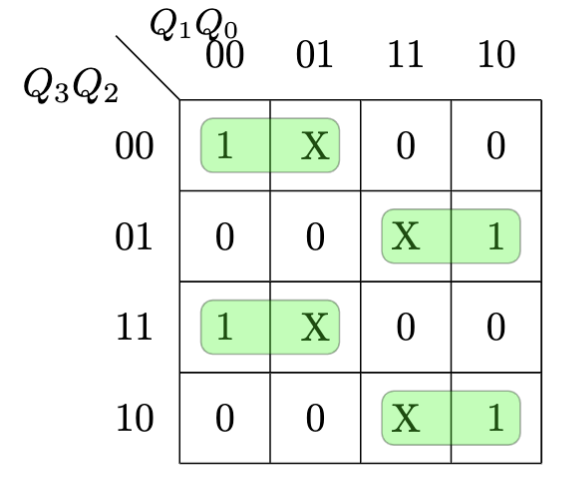
\includegraphics[width=0.6\textwidth]{/q1/s0.png}
        \caption{K-Map for $S_{0}$}
    \end{minipage}
    \begin{minipage}[c]{0.45\textwidth}
        \centering
        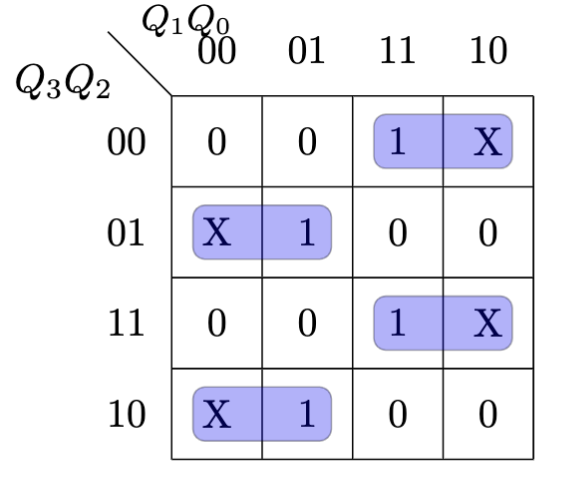
\includegraphics[width=0.6\textwidth]{/q1/r0.png}
        \caption{K-Map for $R_{0}$}
    \end{minipage}
\end{figure}
From the k-maps, for first flipflop, the simplified expressions are $$S_{0} = \bar{Q_{3}}\bar{Q_{2}}\bar{Q_{1}} + \bar{Q_{3}}Q_{2}Q_{1}+\bar{Q_{1}}Q_{2}Q_{3}+\bar{Q_{2}}Q_{3}Q_{1} \implies S_{0} = \bar{Q_{3}}\oplus\bar{Q_{2}}\oplus\bar{Q_{1}}$$
$$R_{0} = \bar{Q_{3}}\bar{Q_{2}}Q_{1} + \bar{Q_{1}}\bar{Q_{2}}Q_{3}+\bar{Q_{3}}\bar{Q_{1}}Q_{2}+Q_{3}Q_{2}Q_{1} \implies R_{0} = Q_{3}\oplus Q_{2}\oplus Q_{1}$$

\begin{figure}[H]
    \centering
    \begin{minipage}[c]{0.45\textwidth}
        \centering
        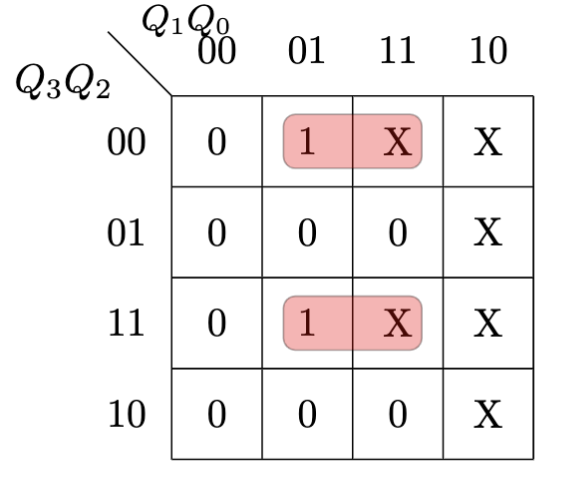
\includegraphics[width=0.6\textwidth]{/q1/s1.png}
        \caption{K-Map for $S_{1}$}
    \end{minipage}
    \begin{minipage}[c]{0.45\textwidth}
        \centering
        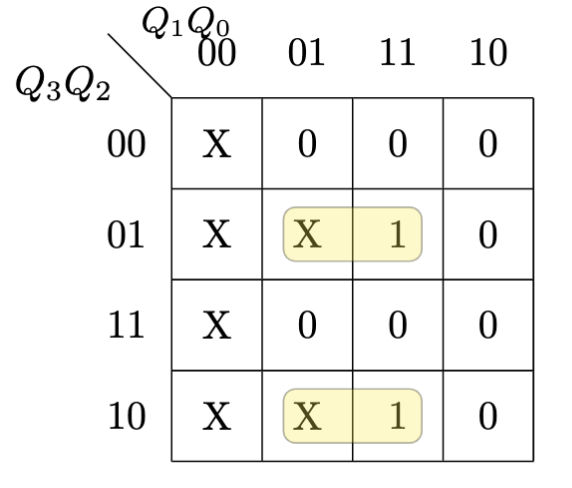
\includegraphics[width=0.6\textwidth]{/q1/r1.png}
        \caption{K-Map for $R_{1}$}
    \end{minipage}
\end{figure}
From the k-maps, for second flipflop, the simplified expressions are
$$ S_{1} = Q_{3}Q_{2}Q_{0}+ \bar{Q_{3}}\bar{Q_{2}}Q_{0} \implies S_{1} = Q_{0}\cdot(\bar{Q_{3}}\oplus Q_{2})$$
$$ R_{1} = \bar{Q_{3}}Q_{2}Q_{0}+ \bar{Q_{2}}Q_{3}Q_{0} \implies R_{1} = Q_{0}\cdot(Q_{3}\oplus Q_{2})$$
\begin{figure}[H]
    \centering
    \begin{minipage}[c]{0.45\textwidth}
        \centering
        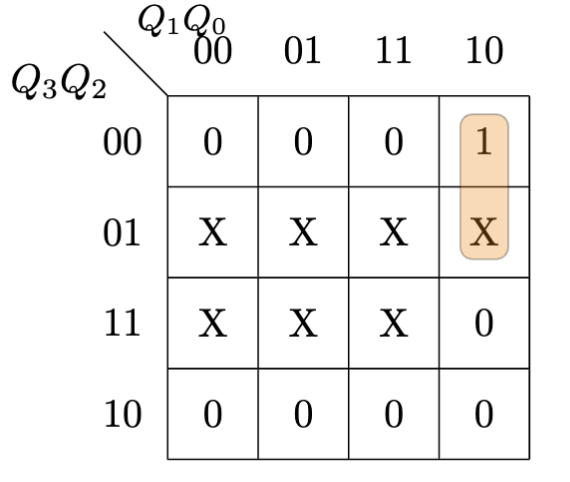
\includegraphics[width=0.6\textwidth]{/q1/s2.png}
        \caption{K-Map for $S_{2}$}
    \end{minipage}
    \begin{minipage}[c]{0.45\textwidth}
        \centering
        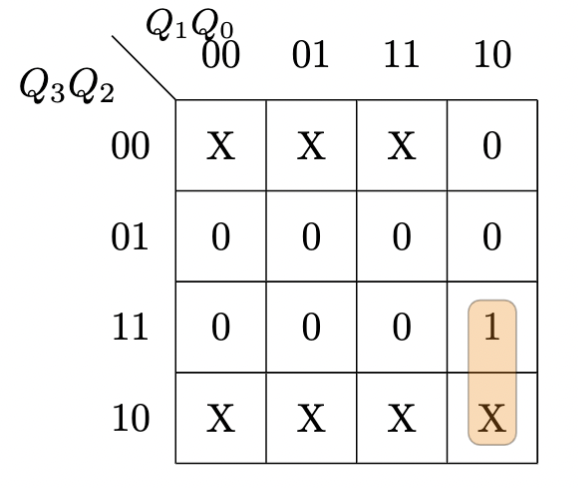
\includegraphics[width=0.6\textwidth]{/q1/r2.png}
        \caption{K-Map for $R_{2}$}
    \end{minipage}
\end{figure}
From the k-maps, for third flipflop, the simplified expressions are
$$S_{2}=\bar{Q_{0}}Q_{1}\bar{Q_{3}}$$
$$R_{2}=\bar{Q_{0}}Q_{1}Q_{3}$$

\begin{figure}[H]
    \centering
    \begin{minipage}[c]{0.45\textwidth}
        \centering
        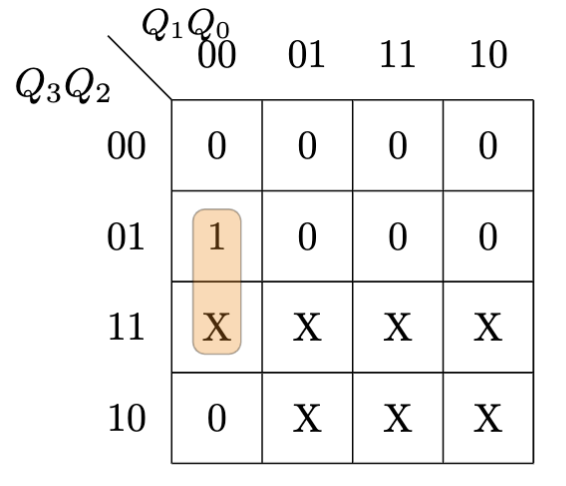
\includegraphics[width=0.6\textwidth]{/q1/s3.png}
        \caption{K-Map for $S_{3}$}
    \end{minipage}
    \begin{minipage}[c]{0.45\textwidth}
        \centering
        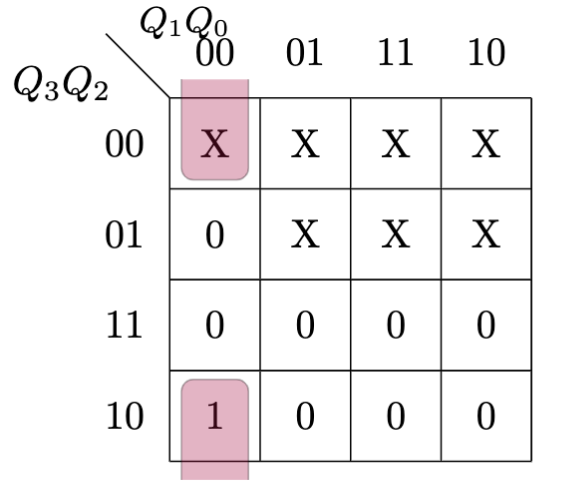
\includegraphics[width=0.6\textwidth]{/q1/r3.png}
        \caption{K-Map for $R_{3}$}
    \end{minipage}
\end{figure}
From the k-maps, for third flipflop, the simplified expressions are
$$S_{3}=Q_{2}\bar{Q_{0}}\bar{Q_{1}}$$
$$R_{3}=\bar{Q_{2}}\bar{Q_{0}}\bar{Q_{1}}$$ \\ \\ \\
\subsection{Circuit Diagram}
The circuit diagram for the counter using the simplified expressions from above, is:
\begin{figure}[H]
    \centering
    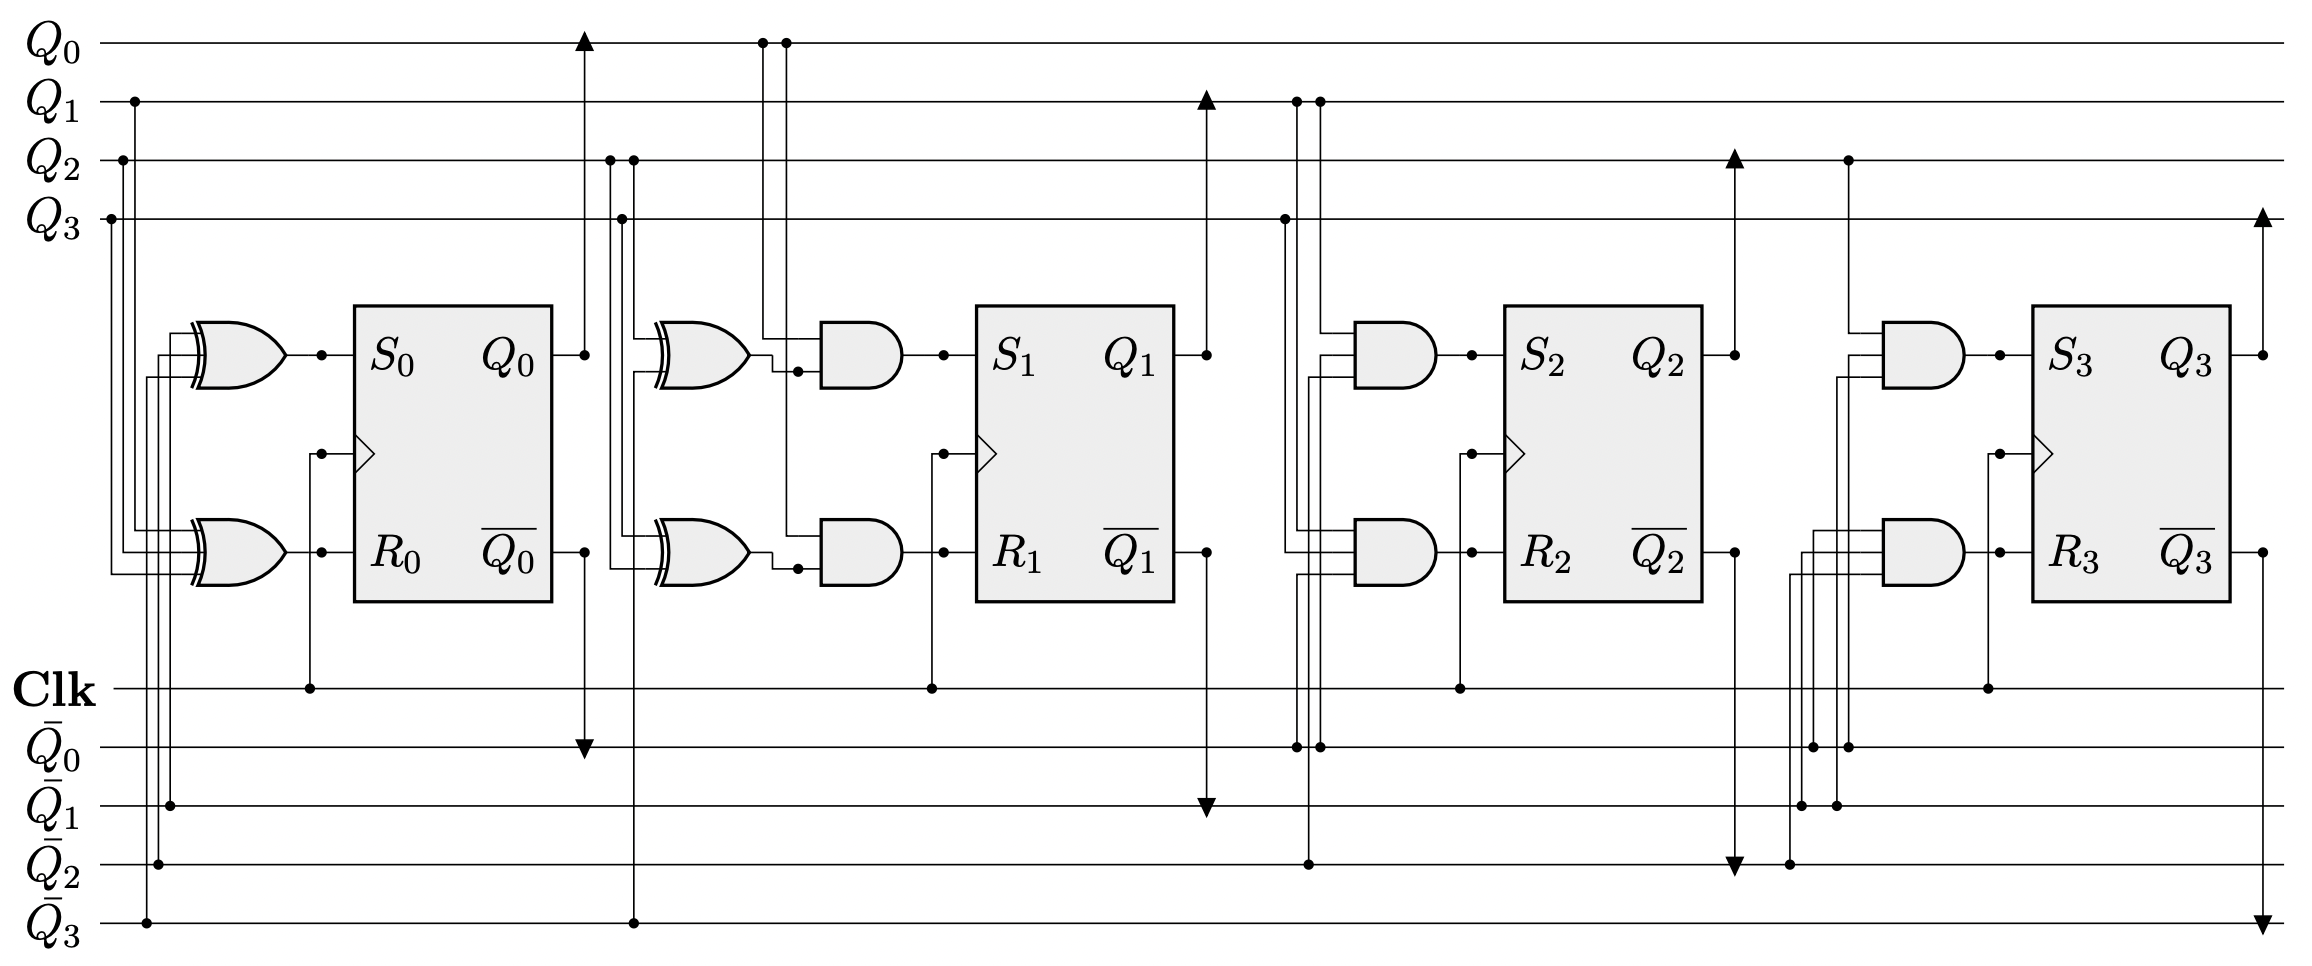
\includegraphics[width=0.99\textwidth]{q1/circuit.png}
    \caption{Circuit Diagram}
\end{figure}
\subsection{Verilog Simulation}
The code is implemented in such a way that flipflops behave as postive edge triggered not latches. 
\subsubsection{Code}
The code for the implementation of the SR flipflop file (design.v) :
\inputminted[bgcolor=bg,frame=lines,framesep=2mm,numbers=left]
{Verilog}{./code-files/q1/design.v} \\
The code for the testbench file (main.v) :
\inputminted[bgcolor=bg,frame=lines,framesep=2mm,numbers=left]
{Verilog}{./code-files/q1/main.v} \\ \\ \\
\subsubsection{Waveform plot}
\begin{figure}[H]
    \centering
    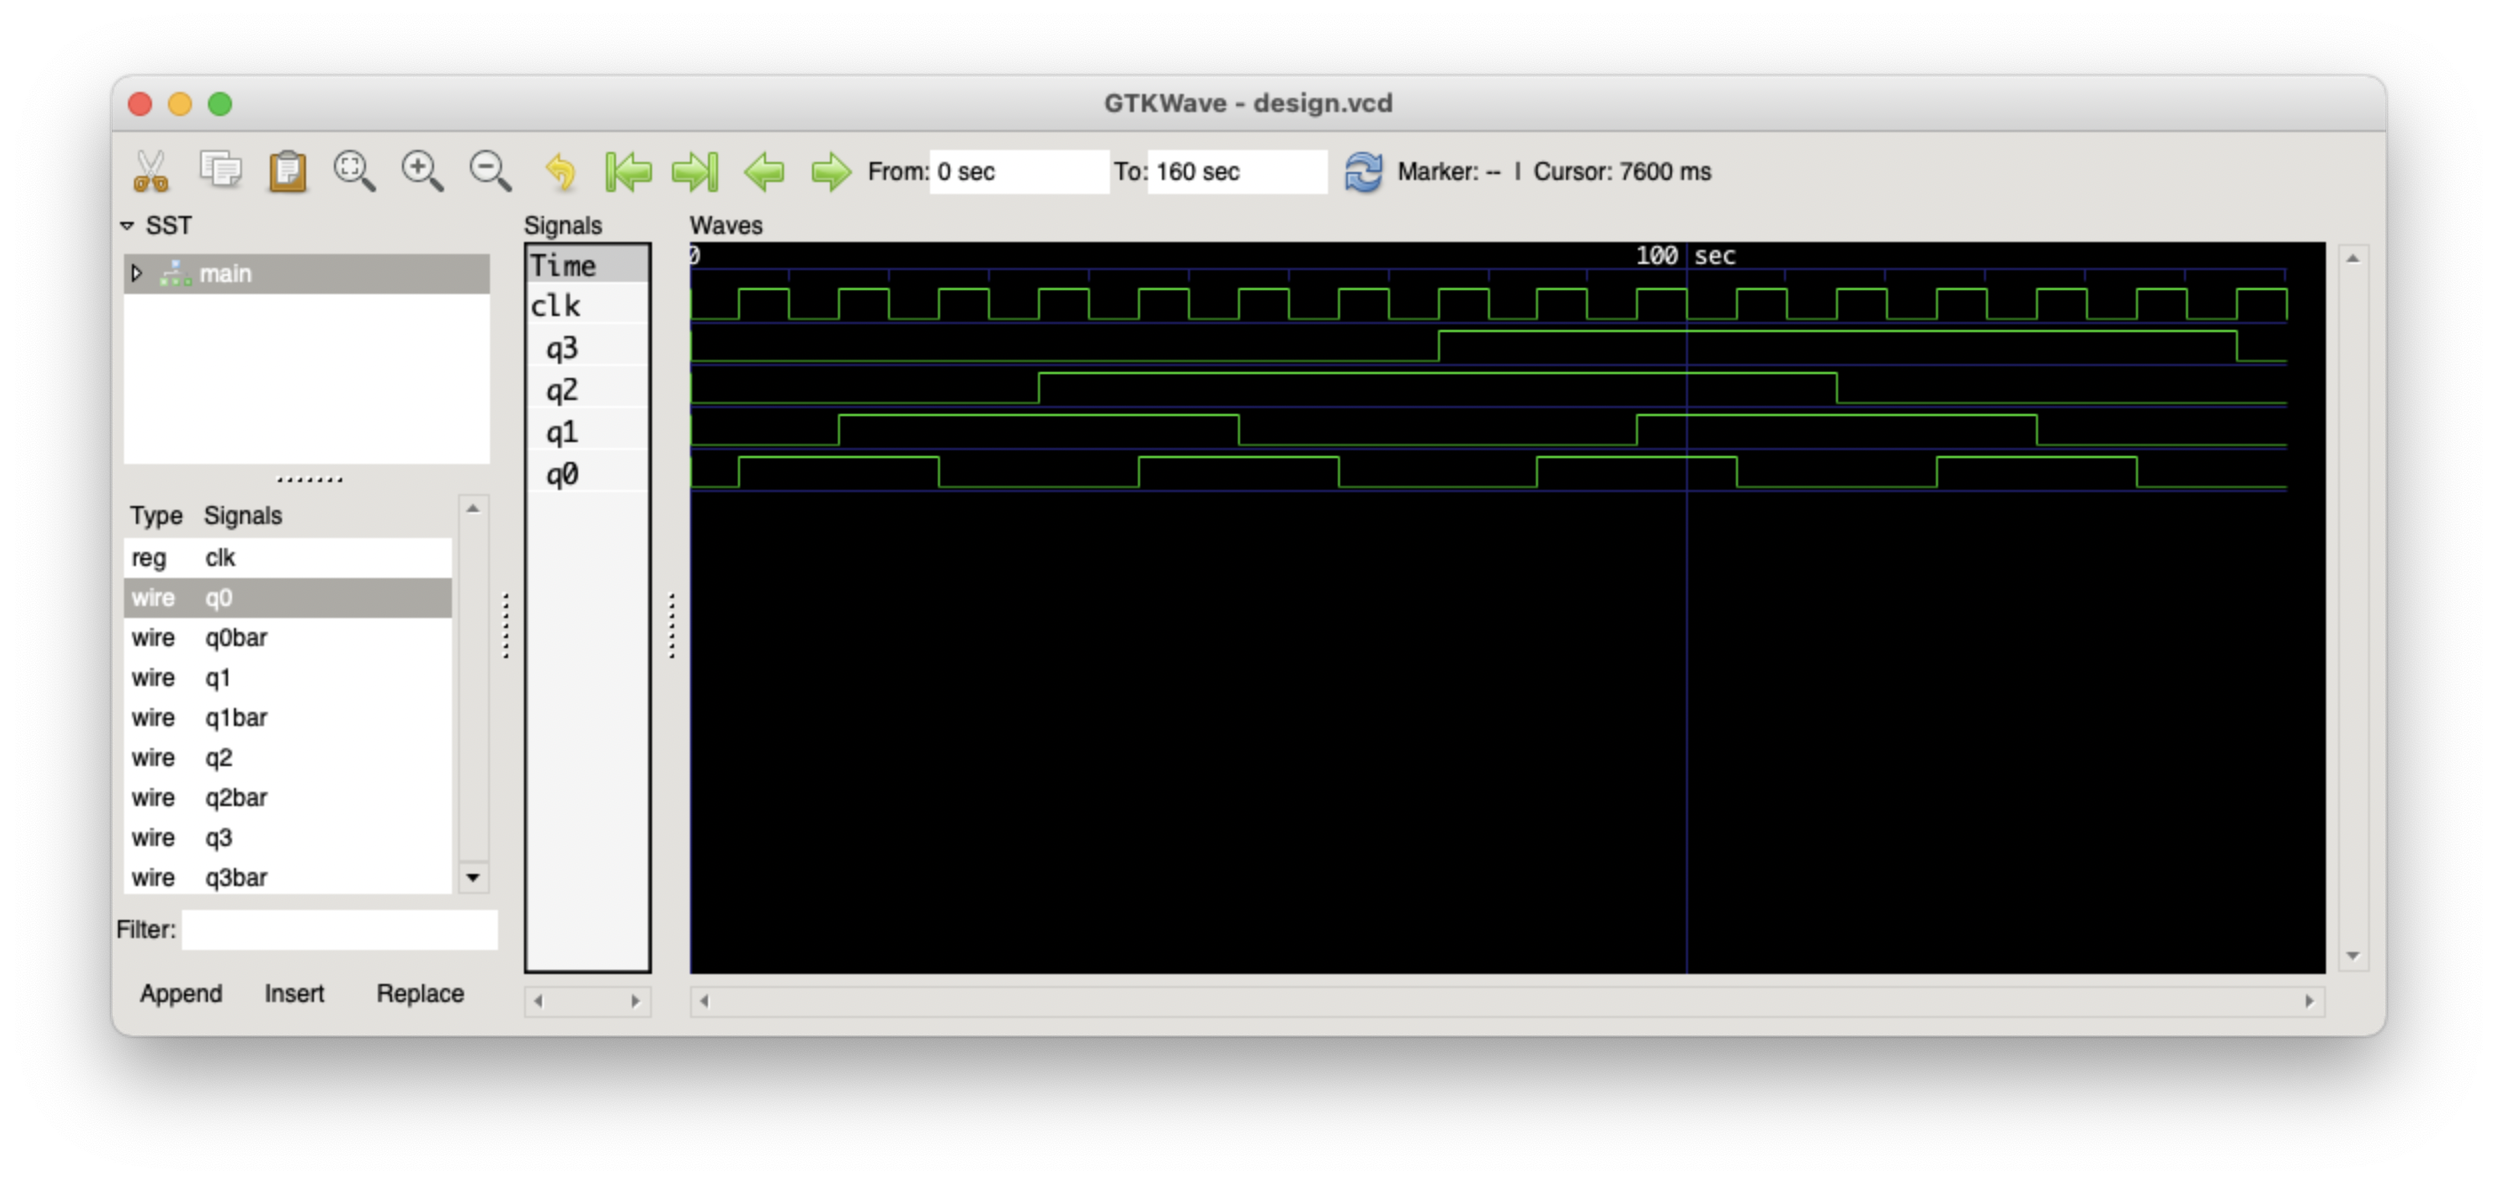
\includegraphics[width=1\textwidth]{/q1/plot.png}
\end{figure}
\section{Synchronous Ring Counter}
\subsection{Introduction}
\begin{wrapfigure}{r}{0.4\linewidth}
    \begin{center}
      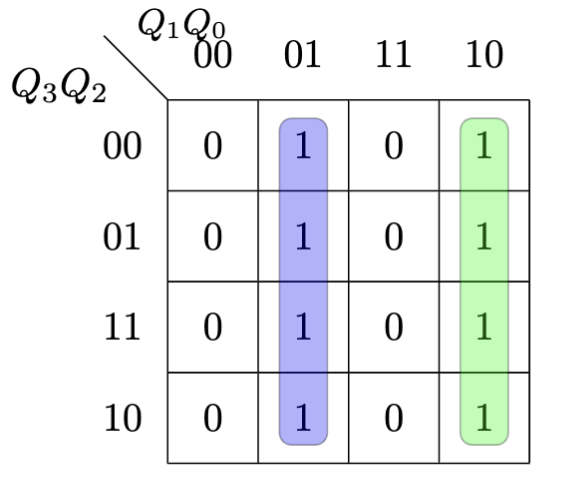
\includegraphics[width=0.3\textwidth]{/q2/kmap.png}
    \end{center}
    \caption{K-Map for $D_{3}$}
  \end{wrapfigure}
From the table it can be observed that there are total 15 different states of the counter. Also since $2^{4} \geq15$, hence total number of D flip-flops required would be 4.

Since the connections for the ring counter are such that for all intermediate flipflops, output of one flipflop is the input for next flipflop, and for the flipflop it can take any combination of the current states. 

Thus from the K-map for $D_{3}$, the simplified expression obtained is : 
$$ D_{3} = Q_{1}\bar{Q_{0}}+Q_{0}\bar{Q_{1}} \implies D_{3} = Q_{1}\oplus Q_{0}$$
\subsection{Circuit Diagram}
Thus the cicuit diagram for this ring counter would be:
\begin{figure}[H]
    \centering
    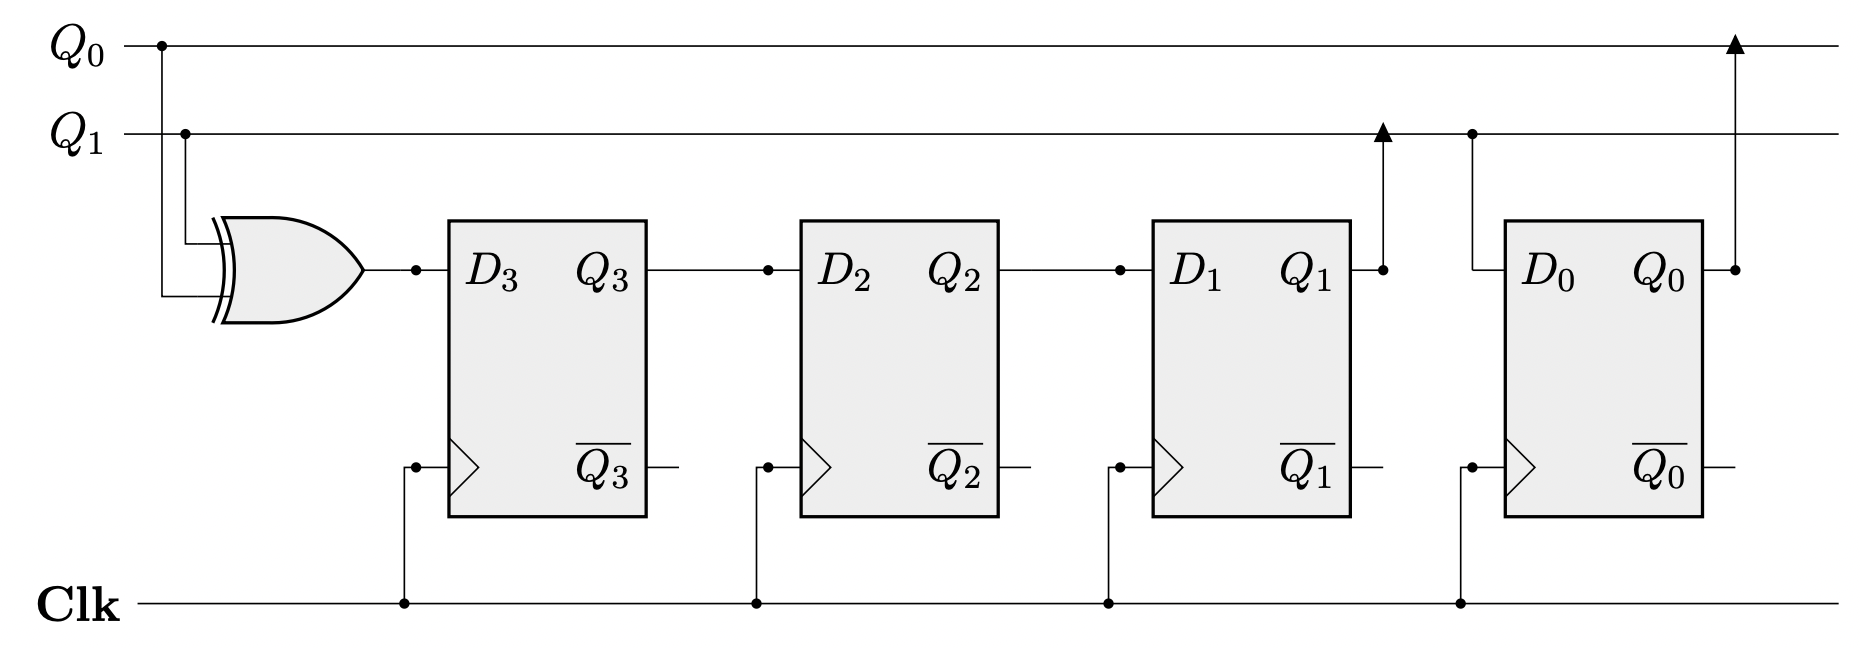
\includegraphics[width=1.1\textwidth]{q2/circuit.png}
    \caption{Circuit Diagram}
\end{figure}
\subsection{Verilog Simulation}
According to my entry number, the initial state should be: 
$$Q_{3}=1 \ ,Q_{2}=0 \ ,Q_{1}=0 \ ,Q_{0}=0$$
The preset parameter is here used to input the initial condition to flipflop. It is configured as low active (hence when preset=0, then $Q=1$). The D flipflops are coded in such a way that they behave as positive edge triggered not latches.
\\ \\ \\ \\ \\ \\ \\ \\ \\ \\ \\
\subsubsection{Code}
The code for the implementation of the D flipflop file (design.v):
\inputminted[bgcolor=bg,frame=lines,framesep=2mm,numbers=left]
{Verilog}{./code-files/q2/design.v}

The code for the testbench file (main.v):
\inputminted[bgcolor=bg,frame=lines,framesep=2mm,numbers=left]
{Verilog}{./code-files/q2/main.v}
\subsubsection{Waveform plot}
\begin{figure}[H]
    \centering
    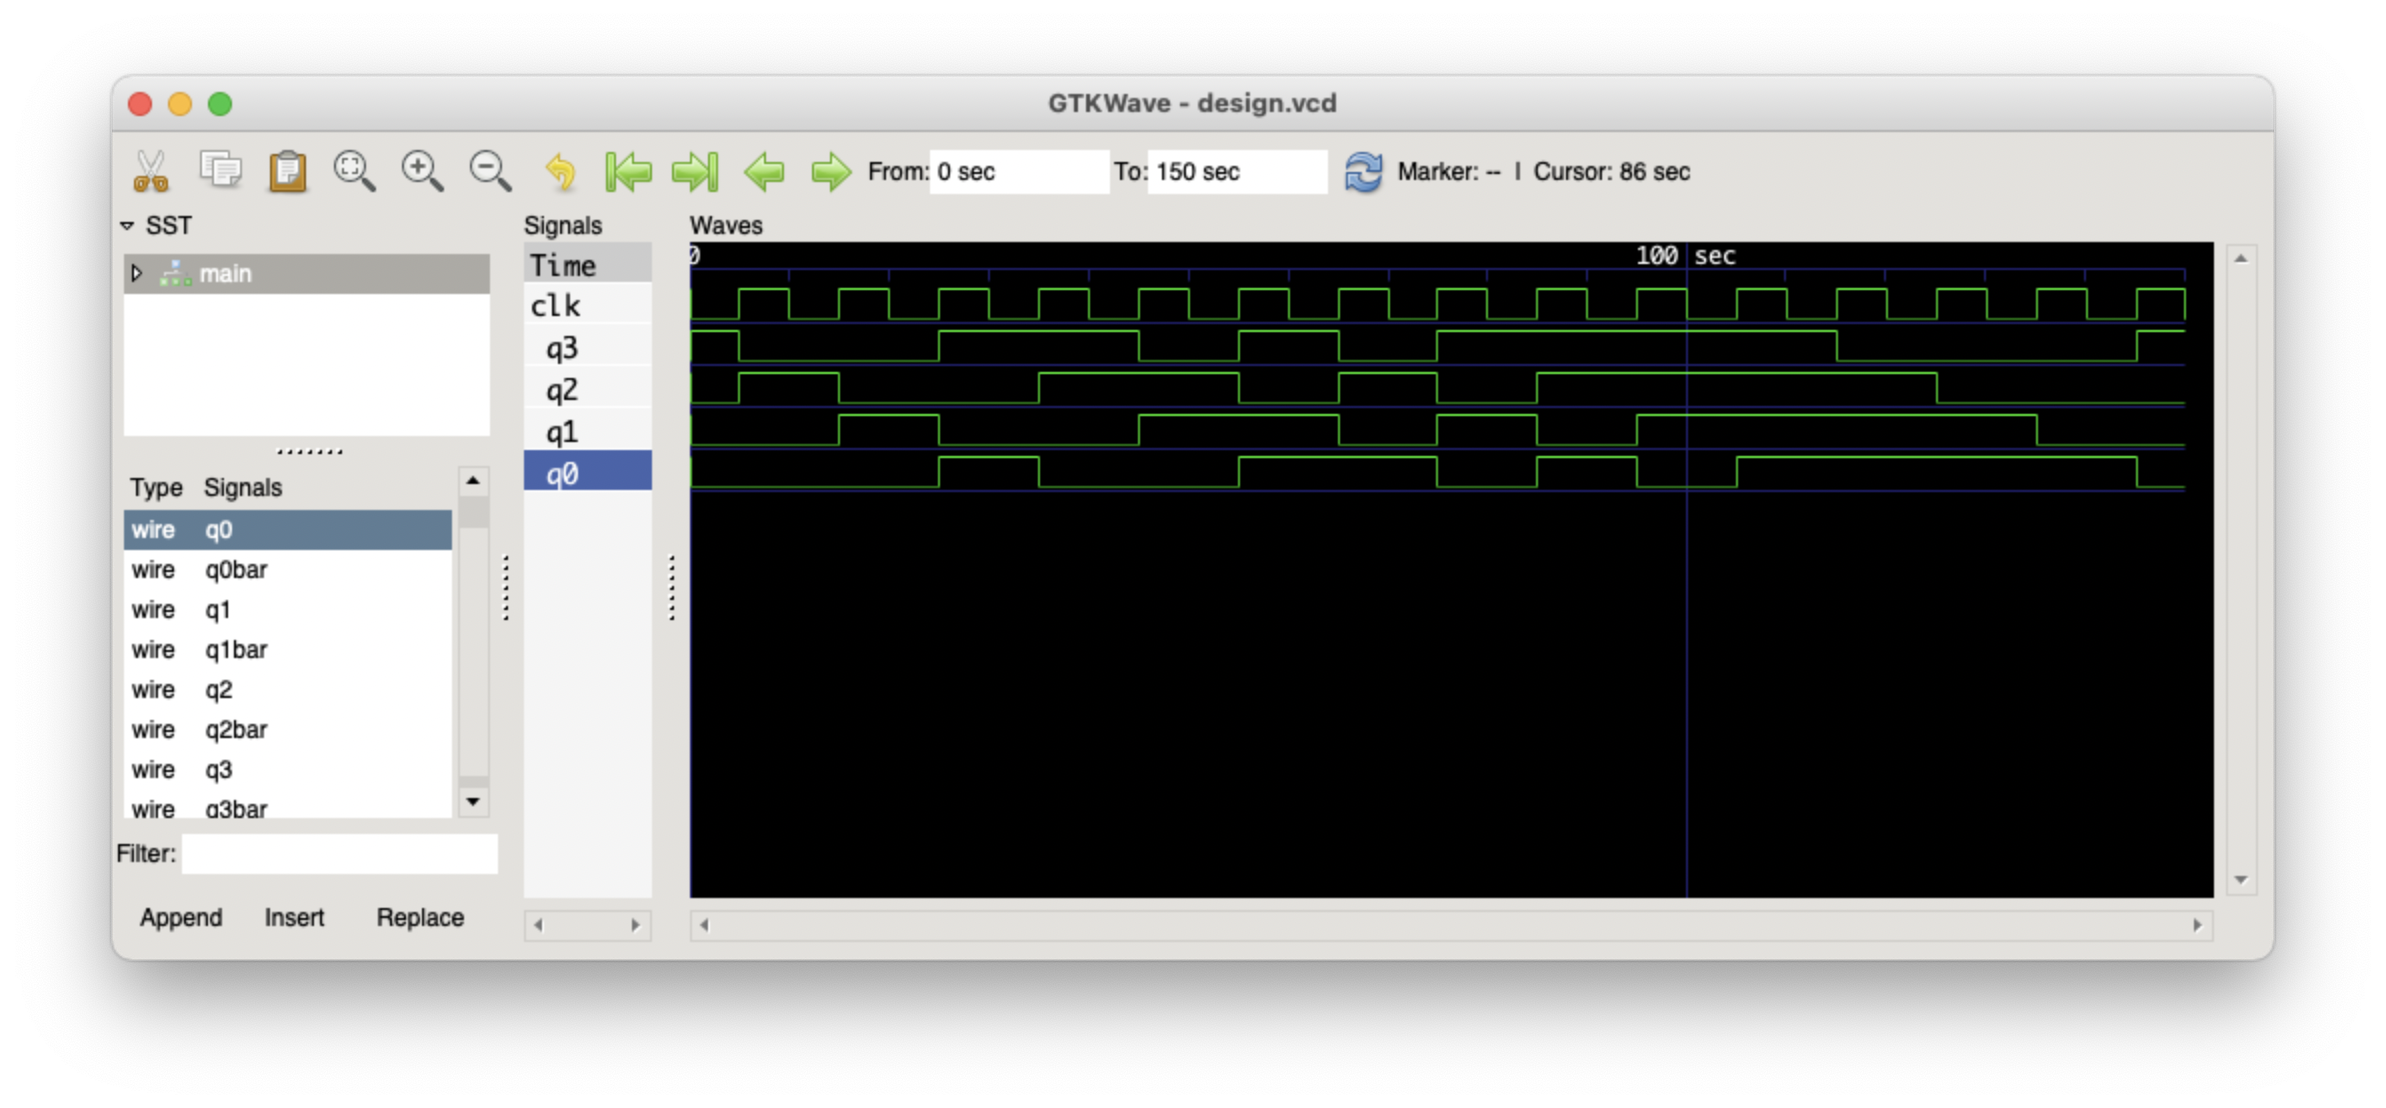
\includegraphics[width=1.1\textwidth]{q2/plot.png}
\end{figure}
\subsection{Further Analysis}
Since the cycle of the counter consists of only 15 states, and the state which isn't getting covered in the cycle is $0000$. If the counter starts from state $0000$, then this state would keep on repeating for every clock impulse and the counter would get stuck in an lockout condition. Whereas if it starts from any other state, then the counter would follow the sequence given in the question, covering each one of the 15 states once before getting back to initial state.
\section{Code Files Link}
The respective code files to run the simulation for both the Synchronous Gray Code Counter and Synchronous Ring Counter can be downloaded from \href{https://drive.google.com/uc?export=download&id=1AyRVoMuTJadTvl_cF-rpAeVn3M3V_eTu}{\textbf{here}}.
\end{document}

% \begin{circuitikz}
%   \ctikzset{logic ports=ieee}
%   \ctikzset{logic ports/fill=mygray}
%   \node (x1) at (-4,0){$Q_{0}$};
%   \node (x2) at (-4,-0.5){$Q_{1}$};
%   \node (x3) at (-4,-1){$Q_{2}$};
%   \node (x4) at (-4,-1.5){$Q_{3}$};

%   \node (clk) at (-4,-5.5){\textbf{Clk}};

%   \node (x5) at (-4,-6){$\bar{Q_{0}}$};
%   \node (x6) at (-4,-6.5){$\bar{Q_{1}}$};
%   \node (x7) at (-4,-7){$\bar{Q_{2}}$};
%   \node (x8) at (-4,-7.5){$\bar{Q_{3}}$};

%   \draw (x1) -- (15,0);
%   \draw (x2) -- (15,-0.5);
%   \draw (x3) -- (15,-1);
%   \draw (x4) -- (15,-1.5);

%   \draw (clk) -- (15,-5.5);
%   \draw (x5) -- (15,-6);
%   \draw (x6) -- (15,-6.5);
%   \draw (x7) -- (15,-7);
%   \draw (x8) -- (15,-7.5);

% 	\node [flipflop SR,
% 		flipflop def={t1=$S_{0}$,t3=$R_{0}$,t6=$Q_{0}$,t4=\ctikztextnot{$Q_{0}$},c2=1},fill=mygray
% 	](ff0) at (-0.6,-3.5){};
% 	\node [flipflop SR,
% 		flipflop def={t1=$S_{1}$,t3=$R_{1}$,t6=$Q_{1}$,t4=\ctikztextnot{$Q_{1}$},c2=1},fill=mygray
% 	](ff1) at (4.7,-3.5){};
% 	\node [flipflop SR,
% 		flipflop def={t1=$S_{2}$,t3=$R_{2}$,t6=$Q_{2}$,t4=\ctikztextnot{$Q_{2}$},c2=1},fill=mygray
% 	](ff2) at (9.2,-3.5){};
% 	\node [flipflop SR,
% 		flipflop def={t1=$S_{3}$,t3=$R_{3}$,t6=$Q_{3}$,t4=\ctikztextnot{$Q_{3}$},c2=1},fill=mygray
% 	](ff3) at (13.7,-3.5){};

%   \draw (ff0.pin 6)node[branch]{} -- (ff0.pin 6 |- x1) node[currarrow,rotate=90]{};
%   \draw (ff1.pin 6)node[branch]{} -- (ff1.pin 6 |- x2) node[currarrow,rotate=90]{};
%   \draw (ff2.pin 6)node[branch]{} -- (ff2.pin 6 |- x3) node[currarrow,rotate=90]{};
%   \draw (ff3.pin 6)node[branch]{} -- (ff3.pin 6 |- x4) node[currarrow,rotate=90]{};

%   \draw (ff0.pin 4)node[branch]{} -- (ff0.pin 4 |- x5) node[currarrow,rotate=-90]{};
%   \draw (ff1.pin 4)node[branch]{} -- (ff1.pin 4 |- x6) node[currarrow,rotate=-90]{};
%   \draw (ff2.pin 4)node[branch]{} -- (ff2.pin 4 |- x7) node[currarrow,rotate=-90]{};
%   \draw (ff3.pin 4)node[branch]{} -- (ff3.pin 4 |- x8) node[currarrow,rotate=-90]{};

%   \node (clk0) at ($(ff0.pin 2)+(-0.1,0)$){};
%   \draw (ff0.pin 2) node[branch]{} -| (clk0 |- clk) node[branch]{};
%   \node (clk1) at ($(ff1.pin 2)+(-0.1,0)$){};
%   \draw (ff1.pin 2) node[branch]{} -| (clk1 |- clk) node[branch]{};
%   \node (clk2) at ($(ff2.pin 2)+(-0.1,0)$){};
%   \draw (ff2.pin 2) node[branch]{} -| (clk2 |- clk) node[branch]{};
%   \node (clk3) at ($(ff3.pin 2)+(-0.1,0)$){};
%   \draw (ff3.pin 2) node[branch]{} -| (clk3 |- clk) node[branch]{};

%   \ctikzset{logic ports/scale=0.5}
%   \node[xor port,draw,number inputs=3] at ($(ff0.pin 1)+(-0.65,0)$) (xor1) {};
%   \node[xor port,draw,number inputs=3] at ($(ff0.pin 3)+(-0.65,0)$) (xor2) {};
%   \node[and port,draw,number inputs=3] at ($(ff2.pin 1)+(-0.65,0)$) (and1) {};
%   \node[and port,draw,number inputs=3] at ($(ff2.pin 3)+(-0.65,0)$) (and2) {};
%   \node[and port,draw,number inputs=3] at ($(ff3.pin 1)+(-0.65,0)$) (and3) {};
%   \node[and port,draw,number inputs=3] at ($(ff3.pin 3)+(-0.65,0)$) (and4) {};
%   \node[xor port,draw] at ($(ff1.pin 1)+(-2,0)$) (xor3) {};
%   \node[and port,draw] at ($(ff1.pin 1)+(-0.7,0)$) (and5) {};
%   \node[xor port,draw] at ($(ff1.pin 3)+(-2,0)$) (xor4) {};
%   \node[and port,draw] at ($(ff1.pin 3)+(-0.7,0)$) (and6) {};

%   \node (temp1) at ($(xor1.in 1)+(-0.1,0)$){}; %connections for ff0
%   \draw (xor1.in 1) -| (temp1 |- x6) node[branch]{};
%   \node (temp2) at ($(xor1.in 2)+(-0.2,0)$){};
%   \draw (xor1.in 2) -| (temp2 |- x7) node[branch]{};
%   \node (temp3) at ($(xor1.in 3)+(-0.3,0)$){};
%   \draw (xor1.in 3) -| (temp3 |- x8) node[branch]{};
%   \node (temp4) at ($(xor2.in 1)+(-0.4,0)$){};
%   \draw (xor2.in 1) -| (temp4 |- x2) node[branch]{};
%   \node (temp5) at ($(xor2.in 2)+(-0.5,0)$){};
%   \draw (xor2.in 2) -| (temp5 |- x3) node[branch]{};
%   \node (temp6) at ($(xor2.in 3)+(-0.6,0)$){};
%   \draw (xor2.in 3) -| (temp6 |- x4) node[branch]{};

%   \node (temp11) at ($(xor3.in 2)+(-0.1,0)$){}; %connections for ff1
%   \draw (xor3.in 2) -| (temp11 |- x8) node[branch]{};
%   \node (temp12) at ($(xor3.in 1)+(-0.1,0)$){};
%   \draw (xor3.in 1) -| (temp12 |- x3) node[branch]{};
%   \node (temp13) at ($(xor4.in 1)+(-0.2,0)$){};
%   \draw (xor4.in 1) -| (temp13 |- x4) node[branch]{};
%   \node (temp14) at ($(xor4.in 2)+(-0.3,0)$){};
%   \draw (xor4.in 2) -| (temp14 |- x3) node[branch]{};
%   \draw (xor3.out) |- (and5.in 2) node[branch]{};
%   \draw (xor4.out) |- (and6.in 2) node[branch]{};
%   \node (temp15) at ($(and6.in 1)+(-0.1,0)$){};
%   \draw (and6.in 1) -| (temp15 |- x1) node[branch]{};
%   \node (temp16) at ($(and5.in 1)+(-0.3,0)$){};
%   \draw (and5.in 1) -| (temp16 |- x1) node[branch]{};

%   \node (temp21) at ($(and1.in 1)+(-0.1,0)$){};
%   \draw (and1.in 1) -| (temp21 |- x2) node[branch]{};
%   \node (temp22) at ($(and1.in 2)+(-0.1,0)$){};
%   \draw (and1.in 2) -| (temp22 |- x5) node[branch]{};
%   \node (temp23) at ($(and1.in 3)+(-0.2,0)$){};
%   \draw (and1.in 3) -| (temp23 |- x7) node[branch]{};
%   \node (temp24) at ($(and2.in 1)+(-0.3,0)$){};
%   \draw (and2.in 1) -| (temp24 |- x2) node[branch]{};
%   \node (temp25) at ($(and2.in 2)+(-0.4,0)$){};
%   \draw (and2.in 2) -| (temp25 |- x4) node[branch]{};
%   \node (temp26) at ($(and2.in 3)+(-0.3,0)$){};
%   \draw (and2.in 3) -| (temp26 |- x5) node[branch]{};

%   \node (temp31) at ($(and3.in 1)+(-0.1,0)$){};
%   \draw (and3.in 1) -| (temp31 |- x3) node[branch]{};
%   \node (temp32) at ($(and3.in 2)+(-0.1,0)$){};
%   \draw (and3.in 2) -| (temp32 |- x5) node[branch]{};
%   \node (temp33) at ($(and3.in 3)+(-0.2,0)$){};
%   \draw (and3.in 3) -| (temp33 |- x6) node[branch]{};
%   \node (temp34) at ($(and3.in 1)+(-0.4,0)$){};
%   \draw (and4.in 1) -| (temp34 |- x5) node[branch]{};
%   \node (temp35) at ($(and3.in 2)+(-0.5,0)$){};
%   \draw (and4.in 2) -| (temp35 |- x6) node[branch]{};
%   \node (temp36) at ($(and3.in 3)+(-0.6,0)$){};
%   \draw (and4.in 3) -| (temp36 |- x7) node[branch]{};

%   \draw (ff0.pin 1)node[branch]{} -| (xor1.out);
%   \draw (ff0.pin 3)node[branch]{} -| (xor2.out);
%   \draw (ff1.pin 1)node[branch]{} -| (and5.out);
%   \draw (ff1.pin 3)node[branch]{} -| (and6.out);
%   \draw (ff2.pin 1)node[branch]{} -| (and1.out);
%   \draw (ff2.pin 3)node[branch]{} -| (and2.out);
%   \draw (ff3.pin 1)node[branch]{} -| (and3.out);
%   \draw (ff3.pin 3)node[branch]{} -| (and4.out);

% \end{circuitikz}


% \begin{circuitikz}
%         \ctikzset{logic ports=ieee}
%         \ctikzset{logic ports/fill=mygray}
%         \ctikzset{multipoles/flipflop/clock wedge size=0.3}
%         \node (clk) at (-4,-2){\textbf{Clk}};
%         \node (x1) at (-4,2){$Q_{1}$};
%         \node (x2) at (-4,2.75){$Q_{0}$};

%         \node [flipflop D,
%             flipflop def={t1=$D_{3}$,t6=$Q_{3}$,t4=\ctikztextnot{$Q_{3}$},c3=1},fill=mygray
%         ](d0) at (0,0){};
%         \node [flipflop D,
%             flipflop def={t1=$D_{2}$,t6=$Q_{2}$,t4=\ctikztextnot{$Q_{2}$},c3=1},fill=mygray
%         ](d1) at (3,0){};
%         \node [flipflop D,
%             flipflop def={t1=$D_{1}$,t6=$Q_{1}$,t4=\ctikztextnot{$Q_{1}$},c3=1},fill=mygray
%         ](d2) at (6,0){};
%         \node [flipflop D,
%             flipflop def={t1=$D_{0}$,t6=$Q_{0}$,t4=\ctikztextnot{$Q_{0}$},c3=1},fill=mygray
%         ](d3) at (9,0){};

%         \draw (clk) -- (11,-2);
%         \draw (x1) -- (11,2);
%         \draw (x2) -- (11,2.75);

%           \node (clk0) at ($(d0.pin 3)+(-0.1,0)$){};
%           \draw (d0.pin 3) node[branch]{} -| (clk0 |- clk) node[branch]{};
%           \node (clk1) at ($(d1.pin 3)+(-0.1,0)$){};
%           \draw (d1.pin 3) node[branch]{} -| (clk1 |- clk) node[branch]{};
%           \node (clk2) at ($(d2.pin 3)+(-0.1,0)$){};
%           \draw (d2.pin 3) node[branch]{} -| (clk2 |- clk) node[branch]{};
%           \node (clk3) at ($(d3.pin 3)+(-0.1,0)$){};
%           \draw (d3.pin 3) node[branch]{} -| (clk3 |- clk) node[branch]{};

%           \draw (d2.pin 6)node[branch]{} -- (d2.pin 6 |- x1) node[currarrow,rotate=90]{};
%           \draw (d3.pin 6)node[branch]{} -- (d3.pin 6 |- x2) node[currarrow,rotate=90]{};

%           \ctikzset{logic ports/scale=0.8}
%           \node[xor port,draw] at ($(d0.pin 1)+(-1,0)$) (xor1) {};

%           \node (temp1) at ($(xor1.in 1)+(-0.1,0)$){};
%           \draw (xor1.in 1) -| (temp1 |- x1) node[branch]{};
%           \node (temp2) at ($(xor1.in 2)+(-0.3,0)$){};
%           \draw (xor1.in 2) -| (temp2 |- x2) node[branch]{};

%           \draw (xor1.out) -| (d0.pin 1)node[branch]{};
%           \draw (d0.pin 6) -| (d1.pin 1)node[branch]{};
%           \draw (d1.pin 6) -| (d2.pin 1)node[branch]{};
%           \draw (d3.pin 1) -| (d3.pin 1 |- x1)node[branch]{};


%     \end{circuitikz}